\appendix
\appendixpage

\section{Derivations}



\subsection{Geometric Etendue}
Geometric etendue is calculated by \cite{Horiba_throughput_etendue}:

\begin{equation}
    d^2G = \frac{dS}{dQ}
\end{equation}

\begin{equation}
    G = \iint\frac{dS}{dQ}
\end{equation}

Where:
\begin{itemize}[label={}]
    \item $G$ [units]: Geometric etendue.
    \item $S$ [units]: Area of the emitting source.
    \item $Q$ [units]: Solid angle into which light propagates (2$\Omega$ in Figure \ref{fig:monochromator}).
\end{itemize}

Through integration:

\begin{equation}
    G = \pi\Sigma\sin^2\Omega
\end{equation}

Where:
\begin{itemize}[label={}]
    \item $G$ [units]: Geometric etendue.
    \item $\Omega$ [units]: Angle of the marginal ray from the optical axis.
\end{itemize}

\subsection{Source \& Image Distances}
\begin{enumerate}[(a)]
    \item In the case of a thin focuser, input rays are parallel, and may be represented by a source that is an infinite distance away. Output rays converge, hence the image is at a finite distance after the lens. Thus:
    \begin{equation}
        \frac{1}{f} = \lim_{d_o\to\infty} \frac{1}{d_o} + \frac{1}{d_i} = \frac{1}{d_i}
    \end{equation}
    
    \begin{equation} \label{eq:image-distance}
        \Rightarrow \ \boxed{d_i = f}    
    \end{equation}
    
    \item In the case of a thin collimator, incoming rays diverge, hence the source is at a finite distance before the lens. Outgoing rays are collimated, which may be represented by an image at an infinite distance away. Thus:
    \begin{equation}
        \frac{1}{f} = \lim_{d_i\to\infty} \frac{1}{d_o} + \frac{1}{d_i} = \frac{1}{d_o}
    \end{equation}
    
    \begin{equation} \label{eq:source-distance}
        \Rightarrow \ \boxed{d_o = f}
    \end{equation}
\end{enumerate}

\subsection{First-Order Model: Thin Lenses in Contact} - move to appendix
\todo{Note: these are Shiqi's derivations. Should be ok but would be good to find source.}

The simplest model assumes lenses are thin and in contact.

Definitions:
\begin{itemize}
    \item $f$: Equivalent focal length of the two lenses.
    \item $f_1$: Focal length of first (convex) lens. Positive.
    \item $f_2$: Focal length of second (concave) lens. Negative.
    \item $s_o$: Object distance of doublet. Equal to object distance of first lens.
    \item $s_i$: Image distance of doublet. Equal to image distance of second lens.
    \item $s_{i,1}$: Image distance of first lens. Equal to object distance of second lens.
\end{itemize}

For first (convex) lens:
\begin{equation}
    \frac{1}{f_1} = \frac{1}{s_o} + \frac{1}{s_{i,1}}
\end{equation}

For second (concave) lens:
\begin{equation}
    \frac{1}{f_2} = -\frac{1}{s_{i,1}} + \frac{1}{s_i}
\end{equation}

Together, by \eqref{eq:achromat-f_eq}:
\begin{align}
    \frac{1}{f} &= \frac{1}{f_1} + \frac{1}{f_2} \\
    &= \frac{1}{s_o} + \frac{1}{s_{i,1}} - \frac{1}{s_{i,1}} + \frac{1}{s_i} \\
    &= \frac{1}{s_o} + \frac{1}{s_i}
\end{align}

This is the Gaussian equation for the thin lens (as in \eqref{eq:thin-lens}), from which object and image distances as well as heights follow. We conclude that this simplified first-order model of an achromatic doublet is equivalent to a thin lens (achromatism is second-order). See Section \ref{sec:thin-singlet-model} for equations as well as their derivations for the focuser and collimator cases.

\textit{Note:} if we modelled the doublet as thin lenses with spacing $d$ between them, we would get the following equivalent focal length $f$ \cite{Boundless_undated-to}:
\begin{equation}
    \frac{1}{f} = \frac{1}{f_1} + \frac{1}{f_2} - \frac{d}{f_1 f_2}
\end{equation}
\textit{}

\section{Constants}
Table \ref{tab:constants} lists the exact values for the scientific constants used in calculations.

\begin{table}[H]
\centering
\caption{Table of constants. Taken from the \href{https://docs.astropy.org/en/stable/constants/index.html}{Astropy} Python package.}
\label{tab:constants}
\begin{tabular}{@{}llll@{}}
\toprule
Constant               & Symbol  & Value                        & Unit                             \\ \midrule
Gravitational Constant & {$G$}   & {\num{6.6743e-11}}           & {\si{\m\cubed\per\kg\s\squared}} \\
Mass of Earth          & {$M_E$} & {\num{5.972167867791379e24}} & {\si{\kg}}                       \\
Planck's Constant      & {$h$}   & {\num{6.62607015e-34}}       & {\si{\joule\s}}                  \\
Radius of Earth        & {$R_E$} & {\num{6378.1}}               & {\si{\km}}                       \\
Speed of Light         & {$c$}   & {\num{299792458}}            & {\si{\m\per\second}}             \\ \bottomrule
\end{tabular}
\end{table}

\subsection{Resolvance} \label{sec:resolvance}
Diffraction gratings have multiple grooves that follow the same relations as a double slit. The expression for resolving power of a grating is derived by using the intensity expression for a double slit grating. 

\begin{figure}[H]
\centering
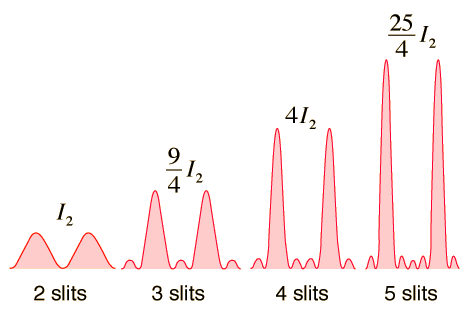
\includegraphics[width=0.5\textwidth]{figures/grating_intensity_curves.png}
\caption{The intensity curves for gratings with varying numbers of slits. Increasing the slits improves the resolution by sharpening the intensity curves.}
\label{fig:grating-intensity}
\end{figure}

The peaks have a phase difference of $\delta$ = 2m$\pi$. The closest minimums occur $\frac{\pi}{2}$ away from the peak, which occurs for a phase change of: 
\begin{equation}
\Delta \delta = \frac{2\pi}{N}
\end{equation}
Where N is the number of slits.

\begin{figure}[H]
\centering
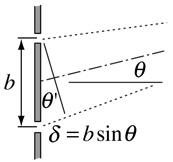
\includegraphics[width=0.5\textwidth]{figures/grating-set-up.png}
\caption{A two-slit grating showing the parameters b, $\theta$, and $\delta$}
\label{fig:grating-set-up}
\end{figure}

From the figure, 
\begin{equation}
\delta = \frac{2\pi}{\lambda}b\sin{\theta}
\end{equation}
The differential of the above is: 
\begin{equation}
d\delta = \frac{2\pi}{\lambda}b\cos{\theta}d\theta
\end{equation}
The maximum condition is:
\begin{equation}
b\sin{\theta} = m\lambda
\end{equation}
With the differential:
\begin{equation}
b\cos{\theta}d\theta = md\lambda
\end{equation}
Substituting both differentials gives:
\begin{equation}
\frac{2\pi}{N} = \frac{2\pi}{\lambda}md\lambda
\end{equation}
This simplifies to the final resolving power formula \cite{Hyperphysics}:
\begin{equation}
\boxed{R = \frac{\lambda}{\Delta \lambda} = mN}
\end{equation}

Where:
\begin{itemize}[label={}]
    \item $\lambda$ is the wavelength of interest.
    \item $\Delta \lambda$ is the resolution.
    \item $m$ is the diffraction order
\end{itemize}